\section{Evaluation} \label{sec:evaluation}


\subsection{Introduction}
The evaluation will be divided into three separate test scenarios. As we are looking into how we can convey weather data through sonification, and how intuitively understood this information compared to visual representations of similar data is. It will be possible to evaluate upon by isolating and comparing data from several tests, where one test is of the produced sonifications, another test with visual elements and one test where both visuals and sonifications is tested. 


More specifically described, a test will be conducted solely where the weather sonifications are presented to test subjects. Similar, a test will be conducted where the visual representations will be presented with the same procedure as the sonification, and finally a test where both visual representations along with the sonification of the data. 
This procedure will make it possible to compare what the test subjects can deduct from the presented data, and allow us to make comparisons towards what information the visual, sonification and combined representations of data is conveying, and thereby make it possible to evaluate upon how well the sonification formulate weather data.

\subsection{Method: Evaluation}
The primary reason of the evaluation is to establish knowledge as to determine if the list of requirements has been fulfilled and to make it possible to gain satisfying results which helps answering to the final problem statement.

The implemented product contains sonifications of specific weather categories, where theese categories has been further categorised into sonifications of different values which represent low, medium and high values of a specific weather category.



\subsection{Hypothesis}

Describe Null and alternative hypothesis.

\subsection{test procedure}

Here are the procedure for the test explained in detail. This chapter will describe the different aspects of the test such as sampling, observations, and guidelines for the testing. The same test procedure will be done on three separate presentations of weather conditions: visual presentation, auditorial representation, and combined presentation.
The general data for the tests are presented below.

Amount of participants: 20 subjects per category per presentation.


Test subject sampling: Convenience sampling: Aalborg university students.


Estimated length of test: 1 minute per subject.


Test location: Area on and around Aalborg university.


Date and time: When appropriate.

\subsubsection{Test Setup}
The test will not require any specific location. 
For the testing only two people are present, i.e. 1 test subject and the test conductor. Only the combined test required two conductors for convenience purposes. The test subject and observer will be placed opposite each other during the test.
Other individuals, in this case other test subjects, will be placed out of view to avoid bias by previous subjects answers.

\subsubsection{Test Materials}
A listing of required materials for each test.
\begin{itemize}
\item Visual Test

\end{itemize}

\subsection{Test results}

\begin{figure}[!htbp]
    \centering
    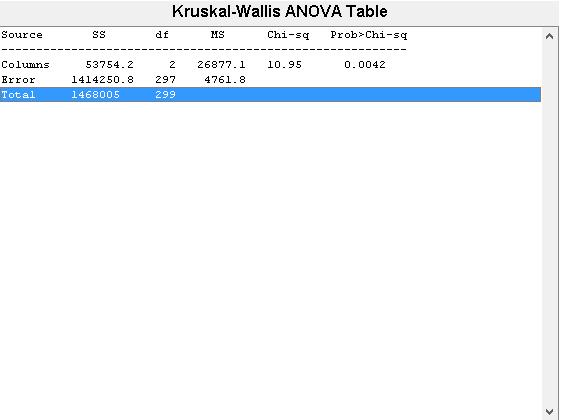
\includegraphics[width=.5\textwidth]{images/tableLow.jpg}
    \caption{Low values: Kruskal-Wallis ANOVA table}
    \label{fig:tableLow}
\end{figure}

\begin{figure}[!htbp]
    \centering
    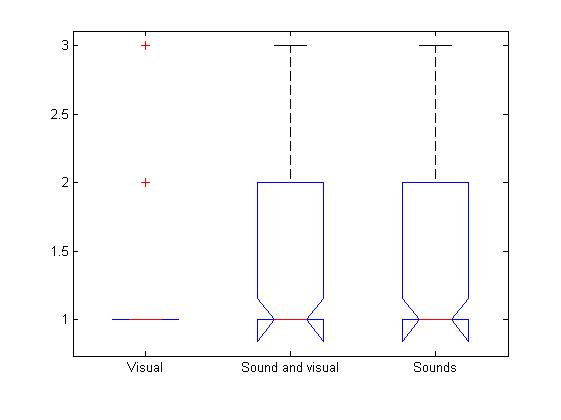
\includegraphics[width=.5\textwidth]{images/boxplotLow.jpg}
    \caption{Low values: Kruskal-Wallis ANOVA Boxplot}
    \label{fig:boxplotLow}
\end{figure}

Generally the boxplot indicates similar levels of medians but the visual scale has a different distribution than "Sound and Visual" and "Sounds".

The "Visual" element is comparatively short, as the inner quartile range is overlapping which suggests that a high number of responses are 1. A majority of participants answered correctly, but a low number of participants, indicated by the "plus", that 2 and 3 was also answered by a lower population of the test participants.

the "Sound and Visual" and "Sounds" indicates similar median...(XX)


\begin{figure}[!htbp]
    \centering
    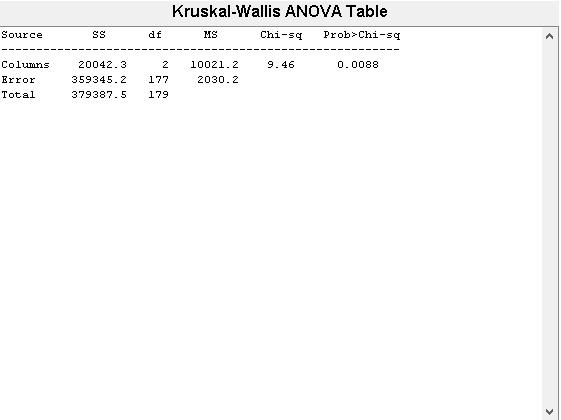
\includegraphics[width=.5\textwidth]{images/tableMiddle.jpg}
    \caption{Middle values: Kruskal-Wallis ANOVA table}
    \label{fig:tableMiddle}
\end{figure}

\begin{figure}[!htbp]
    \centering
    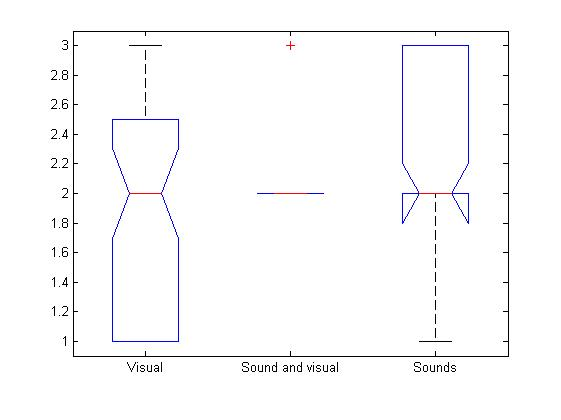
\includegraphics[width=.5\textwidth]{images/boxplotMiddle.jpg}
    \caption{Middle values: Kruskal-Wallis ANOVA Boxplot}
    \label{fig:boxplotMiddle}
\end{figure}

\begin{figure}[!htbp]
    \centering
    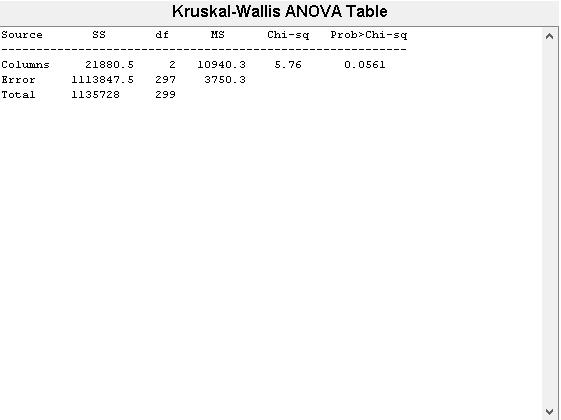
\includegraphics[width=.5\textwidth]{images/tableHigh.jpg}
    \caption{High values: Kruskal-Wallis ANOVA table}
    \label{fig:tableLow}
\end{figure}

\begin{figure}[!htbp]
    \centering
    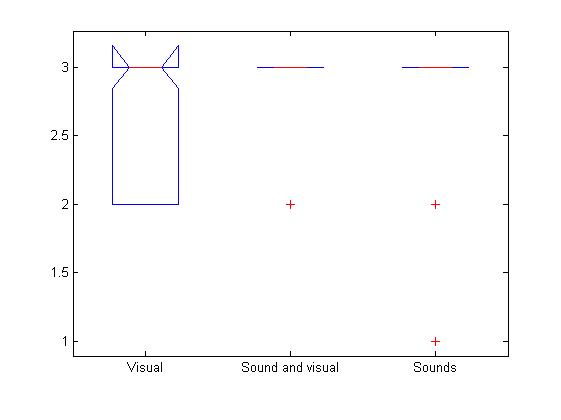
\includegraphics[width=.5\textwidth]{images/boxplotHigh.jpg}
    \caption{High values: Kruskal-Wallis ANOVA Boxplot}
    \label{fig:boxplotHigh}
\end{figure}


\subsection{Test Evaluation}


